

\section{Introduction}


Video inpainting aims to recover the missing content of a corrupted video and assists lots of practical applications,~\emph{e.g.,} video restoration and watermarking removal. 
High-quality video inpainting requires not only realistic structures with visual details but also temporal consistency. 
Though great progress has been made in 2D image inpainting using deep learning techniques \cite{yu2018free,Xiong_2019_CVPR,wang2018high}, directly applying these approaches to each frame individually for video inpainting will lead to flaws, flickers, and jitters due to the additional time dimension. 



Traditional video inpainting methods employ a patch composition framework that composites content in the missing regions via patches by exploiting complementary information across neighboring frames~\cite{patwardhan2007video,wexler2004space,newson2014video}.
% 
These methods rely heavily on the hypothesis that the missing content in the corrupted region appears in neighboring frames, which greatly limits their generalization ability.
%
Recently, deep-learning-based methods have achieved great performance improvement in video inpainting \cite{wang2019video,Kim_2019_CVPR1,Xu_2019_CVPR,Kim_2019_CVPR,lee2019copy,oh2019onion}.
A straightforward solution is to utilize 3D convolution layers to extract spatio-temporal features and predict missing contents with smooth motion \cite{wang2019video}.
To obtain temporally smooth results, contextual information from previous frames is aggregated to synthesize corrupted regions using a recurrent feedback scheme~\cite{Kim_2019_CVPR1,Kim_2019_CVPR}, pixel propagation guided by completed flows~\cite{Xu_2019_CVPR}, or copying similar contents from neighbouring frames \cite{lee2019copy,oh2019onion}.  
By integrating motion guidance, these methods pay more attention to temporal smoothness; however, structure rationality and object details have not been well explored. 


Without definite representation and generation of the target image structures, these methods tend to produce over-smoothed regions. 
Similar observations have been obtained in the image inpainting task \cite{Xiong_2019_CVPR,nazeri2019edgeconnect}.
%\cite{iizuka2017globally,liu2018partialinpainting,yu2018free}. 
To solve this problem, two-step methods are proposed to complete object contours~\cite{Xiong_2019_CVPR} or edge maps~\cite{nazeri2019edgeconnect} first as auxiliary information to guide texture synthesis later in image inpainting.
%
However, when applying these edge-first image inpainting methods to video inpainting, it brings another challenge in generating temporally coherent structures while human vision is significantly sensitive to temporal discontinuity that frequently occurs at edges. 


In order to simultaneously hallucinate detailed image structures and preserve temporal coherence in video inpainting, we present a novel structure-guided video inpainting approach which effectively exploits the spatio-temporal structure information to improve the quality of video inpainting.  
%
Compared with previous video inpainting methods that only consider motion guidance, we explore the correlation between structure, texture, and motion to complete the missing region with reasonable structure, rich visual details, and temporal coherence, as shown in Fig.~\ref{fig:overview}.
% first, edge -- structure
First, we design an edge inpainting network (ENet) to predict sparse edges in the missing region to represent the target structure for each frame by exploiting the spatio-temporal neighboring information from adjacent frames.
%Second, texture
Then, under the guidance of completed edges, we employ a texture inpainting network (TexNet) to fill the missing region via a coarse-to-fine architecture and a structure attention module (SAM).
Specifically, the SAM is designed to guide the texture generation by capturing the latent spatial relevance between video textures and the synthesized edges.
Notably, such a structure-texture relevance can effectively improve the inpainting quality in TexNet with fewer cracks and more realistic object contours.
Furthermore, to enhance the temporal coherence of synthesized frames, we employ motion flows for consistency check of both edge maps and inpainted frames during the training stage.
%
The ground truth optical flow is exploited to guide both ENet and TexNet to generate temporally smooth edge maps and texture results via edge consistency and frame warping losses.
Consequently, the inpainted frames using our approach are not only temporally consistent, but also more complete in structure and rich in visual details.
 

%In summary, we present a novel structure-guided video inpainting method, which can generate structural reasonable and temporal coherent inpainted frames.
%
We conduct a series of experiments on the YouTubeVOS and DAVIS datasets under various mask settings. 
The results show that the proposed method obtains new state-of-the-art inpainting performance both quantitatively and qualitatively. 
%Because of the sparsity of edge maps, the computational cost is also greatly reduced.
In summary, our technical contributions are three-fold:
\begin{itemize}
	\item We propose a novel structure-guided video inpainting method which integrates scene structure, texture, and motion to complete the missing region with realistic structure, rich visual details, and temporal coherence.
	% explore the correlation 	
	\item A structure attention module is designed to capture the correlation between hallucinated edges and video textures, which can provide better structural guidance for texture synthesis. % edge - texture 
	\item Flow-guided edge and frame consistency constraints are developed to enhance the temporal coherence of both completed edges and video frames.   
\end{itemize}


%The rest of this paper is organized as follows. Section~\ref{sec:rw} reviews the related works. Section~\ref{sec:approach} illustrates the proposed video inpainting method. Section~\ref{sec:exp} provides the experiments on YouTubeVOS and DAVIS datasets, and Section~\ref{sec:conclu} concludes the whole paper.


\begin{figure}[t]
	\centering
	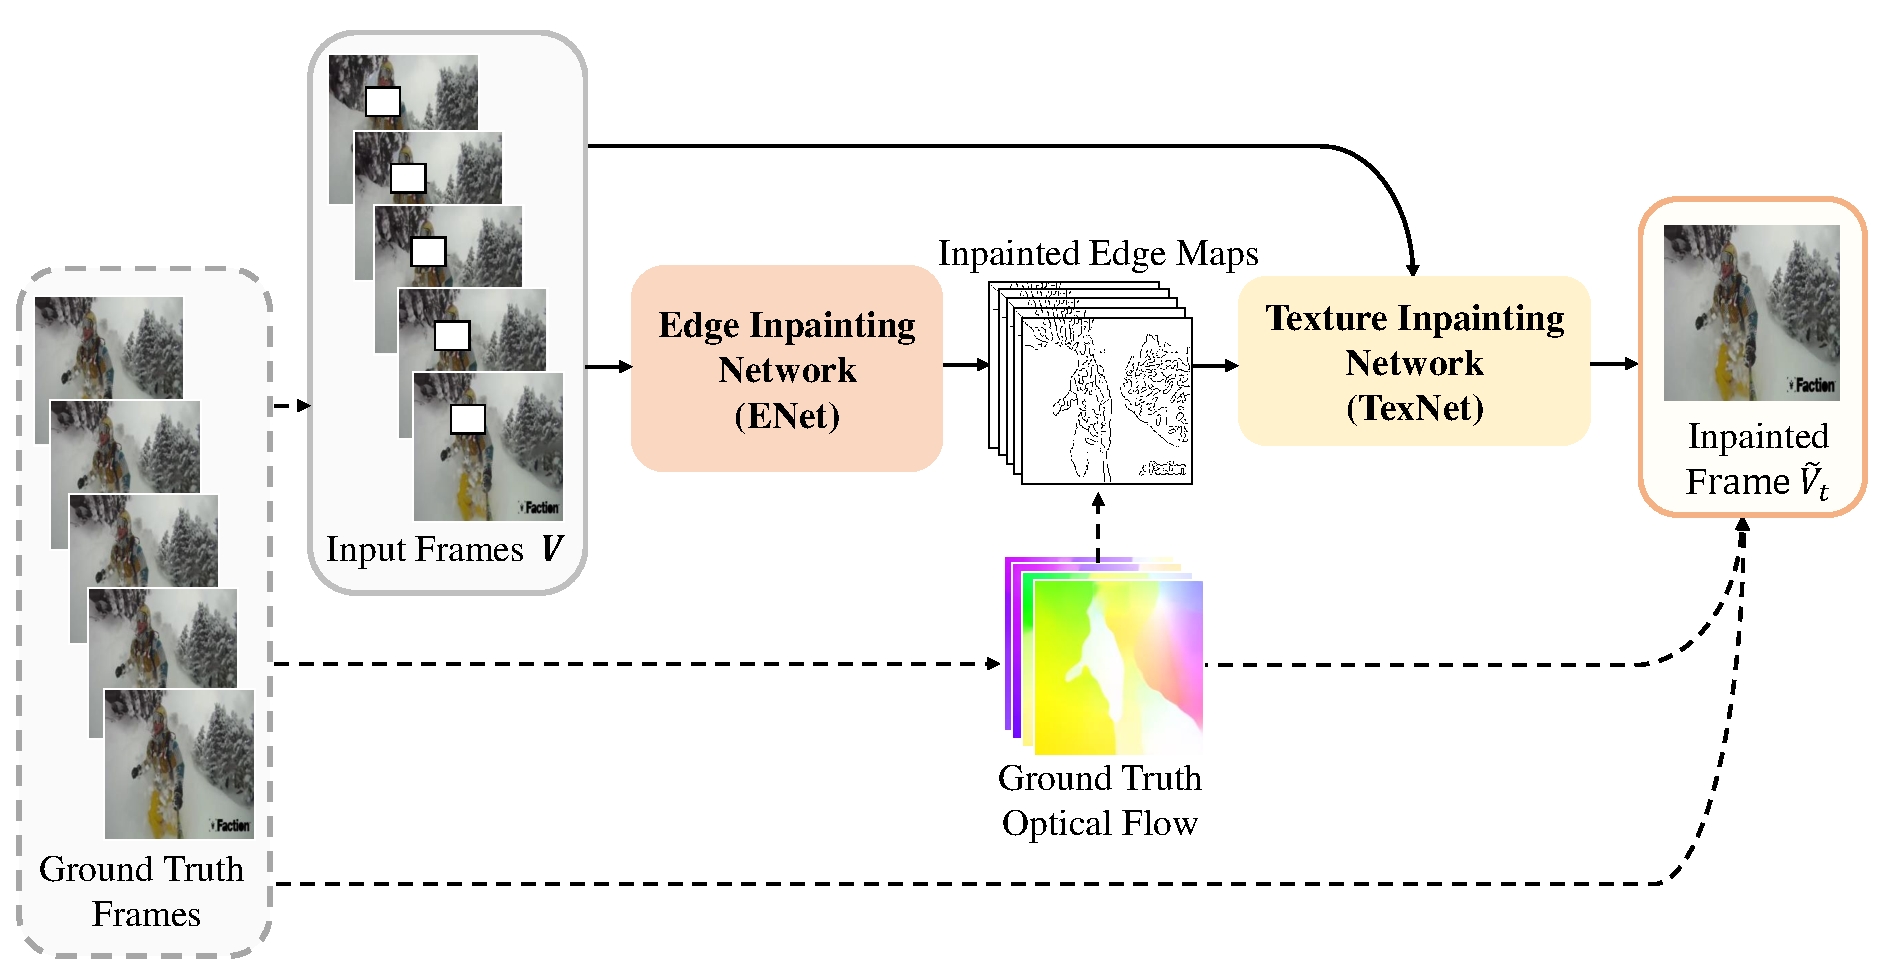
\includegraphics[width=1.01\columnwidth]{pipeline} 
	\caption{Overview of our structure-guided video inpainting network. We first complete the edges in the corrupted region by aggregating information from neighboring frames to represent the target structure using the ENet. Then, the TexNet synthesizes missing textures under the structural guidance of inpainted edges. Besides, the ground truth optical flow between frames is utilized during the training stage for both ENet and TexNet to enforce temporal coherence of completed contents, as illustrated by dotted lines.}
	\label{fig:overview}
\end{figure}






\section{Related Work}

%
\mdf{Image and video inpainting has been studied for decades. In this section, we mainly discuss four categories of related works, including (a) traditional methods of image inpainting, (b) patch-based video inpainting, (c) CNN-based image inpainting, and (d) deep video inpainting.  }


\paragraph{Traditional Image Inpainting Approaches}
Traditional methods of image and video inpainting can be divided into two categories, diffusion-based and patch-based methods. 
Diffusion-based methods \cite{bertalmio2000image,ballester2001filling,sridevi2019image} gradually propagate contents from surrounding areas to the missing region. 
%Li \emph{et al.}~\cite{li2016image} define diffusion coefficients according to the relation between the damaged pixels and neighborhood pixels.
%Li \emph{et al.}~\cite{li2017localization} attempt to solve the problem of localization of diffusion-based inpainted regions.
%Fractional-order nonlinear diffusion driven by difference curvature is proposed to produce clearer image details \cite{sridevi2019image}. 
However, this category of methods fail to handle large holes due to its assumption of local smoothness. 
%
Patch-based image inpainting methods, also called exemplar-based methods~\cite{bertalmio2003simultaneous,efros2001image,li2008patch,zhang2014image}, are more widely studied.
They formulate the completion task as a patch-based optimization problem. 
Barnes \emph{et al.}~\cite{barnes2009patchmatch} employ approximate nearest neighbor algorithm to fill the damaged regions.
Sangeetha \emph{et al.}~\cite{sangeetha2011combined} propose to propagate both linear structure and two-dimensional texture into the target region.
Ru{\v{z}}i{\'c} \emph{et al.} \cite{ruvzic2014context} introduce Markov random field to search the most matched candidates.
Ding \emph{et al.} \cite{ding_19nonlocal} employ nonlocal texture similarity and local intensity smoothness to produce natural-looking results.
Besides, some patch-based methods utilize low rank approximation. For example, Guo \emph{et al.} \cite{pb_lowrank2018} propose a simple two-stage low rank approximation to recover the corrupted region, which avoids time-consuming iterations.
Lu \emph{et al.} \cite{lu2018gradient} adopt gradient-based low rank approximation.
These patch-based methods fill the missing content by borrowing and aggregating the most similar patches based on low-level image features from known regions. However, they usually fail when there is insufficient information in known regions or image textures are too complicated.  
%

\paragraph{Patch-Based Video Inpainting} Patch-based methods are also widely studied for video inpainting \cite{wexler2007space,tcsvt2009,umeda2012removal,xu2015video}. 
They search similar patches and borrow appearances from known regions across neighboring frames to synthesize the unknown content. 
Wexler \emph{et al.} \cite{wexler2007space} constrain masked regions to synthesize coherent structures with respect to reference examples based on local structures. 
Umeda \emph{et al.} \cite{umeda2012removal} propose using directional median filter as complementation of patch-based filling.
Newson \emph{et al.} \cite{newson2014video} extend the 2D PatchMatch algorithm~\cite{barnes2009patchmatch} into 3D version to improve video inpainting quality.
Xu \emph{et al.} \cite{xu2015video} first complete motion field to guide the patch composition for video background completion.
Huang \emph{et al.} \cite{huang2016temporally} jointly estimate optical flow and textures to promote temporal coherence.
%
Another group of methods separate foreground and background apart, and then deal with the two parts respectively with different algorithms, since there naturally exists property difference between them.  
Ghanbari \emph{et al.} \cite{ghanbari2011contour} first separate foreground and background in videos, and fills the two parts accordingly with the help of contours.
Xia \emph{et al.} \cite{xia2011exemplar} make use of Gaussian mixture models to distinguish moving foreground and still background, and process them separately.   
%However, traditional metshods assume that there exist similar contents in known regions, thus fail to synthesize unseen appearances. 
However, in these patch-based video inpainting methods, the patch-searching process suffers from high computational complexity, thus limits their usage in practical applications.



\begin{figure*}[!t]
	\centering
	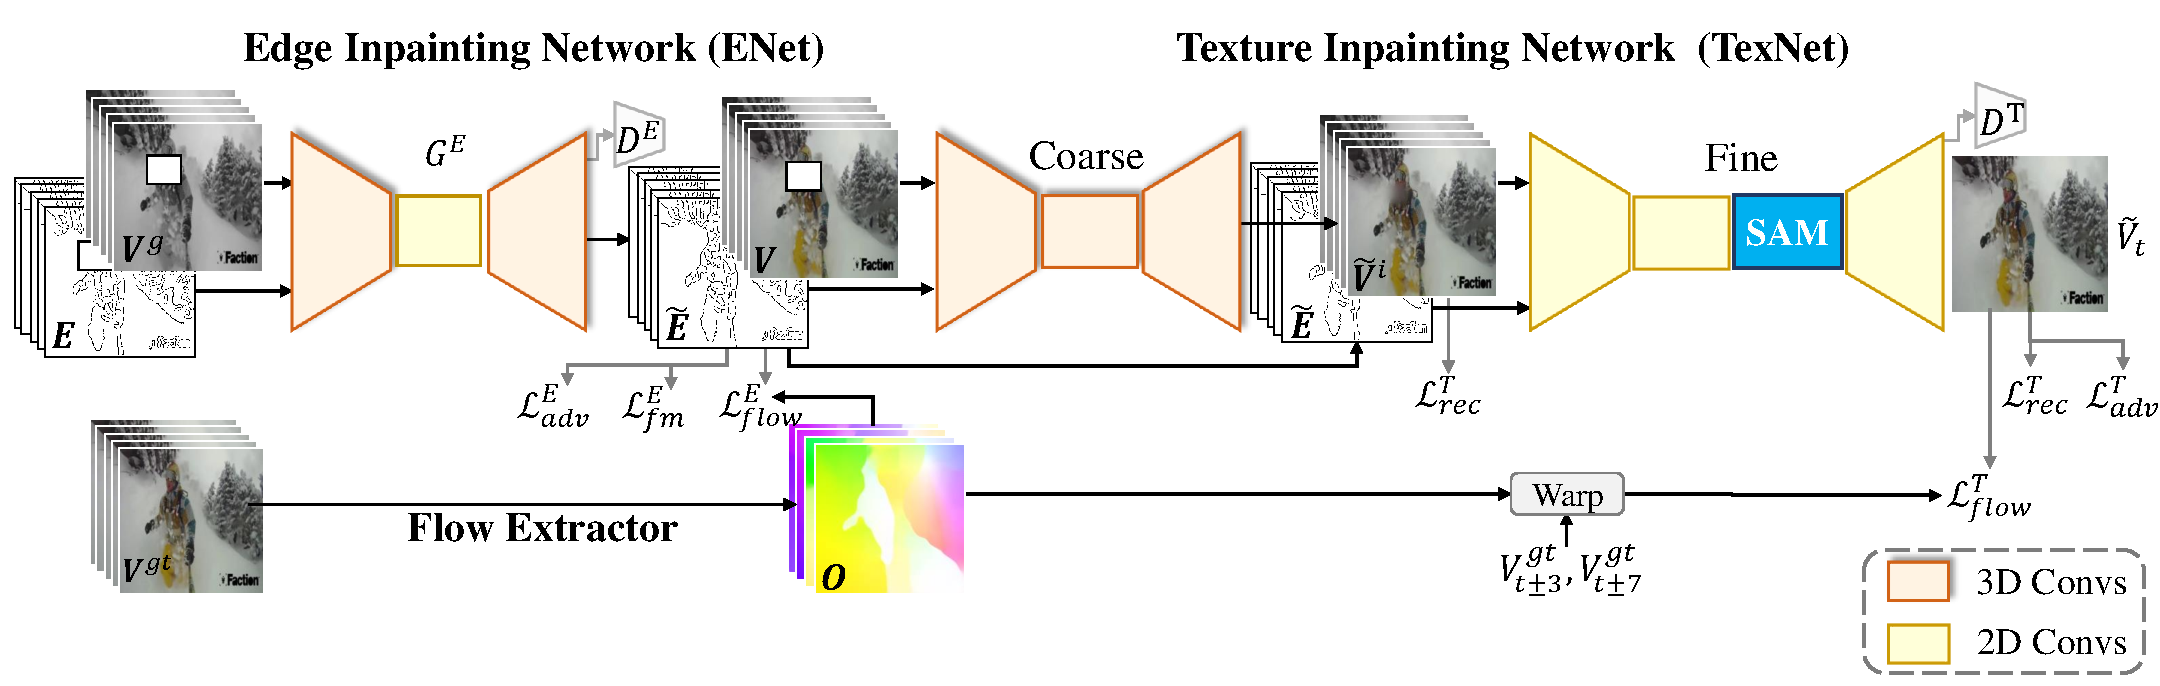
\includegraphics[width=2.05\columnwidth]{sti} % 
	\caption{The detailed architecture of our network. ENet adopts an encoder-decoder architecture to complete edges in the missing regions. TexNet utilizes a coarse-to-fine manner to inpaint the final frames. Ground truth optical flow between adjacent frames is employed in edge consistency loss and frame warping loss to enforce temporal coherence. }
	\label{fig:stiNet}
\end{figure*}

\paragraph{CNN-based Image Inpainting}
Recently, deep learning methods have achieved tremendous progress in the field
of computer vision. The tasks of image and video inpainting also have witnessed great promotion thanks to the capability of deep neural networks to capture high-level semantic information in images and videos.
%
A convolution neural network (CNN) is first introduced to directly synthesize image contents in the masked regions for image denoising and inpainting in \cite{xie2012image}.
To improve the photorealism of the synthesized content, a generative adversarial network is employed \cite{pathak2016context}. 
Then, Yang \emph{et al.} \cite{yang2017high} take advantages of multi-scale representation to boost details generation.
%by jointly training a generator and a discriminator in a minimax manner. 
Multiple discriminators are used to constrain both global and local coherence of image contents \cite{iizuka2017globally}.  
Yu \emph{et al.} \cite{yu2018generative} propose a contextual attention module in capturing long-range information.
Subsequent approaches solve more specific problems in image inpainting, for example, inpainting irregular holes with partial convolution~\cite{liu2018partialinpainting} or employing gated convolution \cite{yu2018free} for dynamic feature selection. 
While these methods tend to generate over-smoothed and blurry results, a two-stage approach is proposed to hallucinate edges first and then fill image colors using the edges as a prior \cite{nazeri2019edgeconnect}. 
Similarly, Xiong \emph{et al.} \cite{Xiong_2019_CVPR} predict contours of foreground objects to guide the inpainting process of masked regions.
Though high-quality static images with reasonable structure can be generated using these edge-based methods, simply extending it from image inpainting to video inpainting by 3D convolutions inevitably fails because of no guarantee on the temporal coherence, especially on the high-frequency signals. 
Besides, these methods simply utilize edges and contours as one additional channel of the image inpainting network, without exploiting the mutual relationship between edges and textures. 
In comparison, we design a structure attention module to better explore the structural guidance in synthesizing textures. 


%%% video inpainting 
\paragraph{Deep Video Inpainting}
Several video inpainting methods based on deep neural networks have been proposed recently, to fully utilize useful complementary information in neighboring frames.
%
The first deep-learning-based video inpainting method is CombCN \cite{wang2019video}, which jointly learns temporal structure and spatial details via 3D convolutions.
%%\cite{Xu_2019_CVPR} proposes a stacked convolution network to predict missing motion field and regards video inpainting as a pixel propagation problem. 
%
To enforce temporal coherence, features from neighboring frames are collected and refined to synthesize the missing content with recurrent feedback \cite{Kim_2019_CVPR1,Kim_2019_CVPR}. 
\mdf{OPN \cite{oh2019onion} uses the non-local formulation to calculate the similarity between pixels in reference and target frames, and then copies the contents based on the similarity.
%The similarity is between video contents.
Similarly, Copy-and-Paste \cite{lee2019copy} copies matching contexts in aligned reference frames and pastes them to the corrupted region.
However, both OPN and Copy-and-Paste only consider the texture correlation between neighboring frames, while ignoring high-level structures.
In comparison, we explore the correlation between structures and textures to achieve high-quality inpainting results.}  
%
Instead of filling pixel colors directly using CNNs, flow a deep flow-guided inpainting network is proposed to estimate optical flow first in the missing region and then propagate pixel colors based on the completed flow \cite{Xu_2019_CVPR}.
However, these existing methods usually suffer from blurs and structural cracks in the synthesized frames since it is non-trivial to maintain fine details and sharp edges simultaneously when predicting temporally coherent pixel colors. 
In comparison, we propose to explicitly complete the target structure using edges, which are efficient due to their sparsity. To utilize structural information more effectively, we also introduce a structure attention mechanism. 
Under the structural guidance, more visually pleasing results could be synthesized with plausible structure and fine details. 

 



























